\newpage

\subsubsection*{\textbf{Тест}: <<Удаление элемента из таблицы MySQL через таблицу на сайте>>}

\underline{Ожидаемый результат}:
Из таблицы MySQL удалиться элемент, который был удален при нажатии иконки <<Корзина>> в таблице на сайте.

\underline{Описание}:
Тестирование правильности удаления элемента из таблицы MySQL через таблицу на сайте, по нажатию иконки <<корзина>>.

\underline{Полученный результат}:

\begin{itemize}
    \item Таблица phpmyadmin до удаления элемента
    на рисунке \ref{fig:mysql_table_after}
    (стр. \pageref{fig:mysql_table_after}).

    \item Вывод таблицы на сайте до удаления элемента
    на рисунке \ref{fig:site_table_after}
    (стр. \pageref{fig:site_table_after}).

    \item Таблица MySQL после удаления элемента
    на рисунке \ref{fig:mysql_table_after_deleting}
    (стр. \pageref{fig:mysql_table_after_deleting}).

    \item Вывод таблицы на сайте после удаления элемента
    на рисунке \ref{fig:site_table_after_deleting}
    (стр. \pageref{fig:site_table_after_deleting}).
\end{itemize}

\begin{figure}[p]
    \center{
        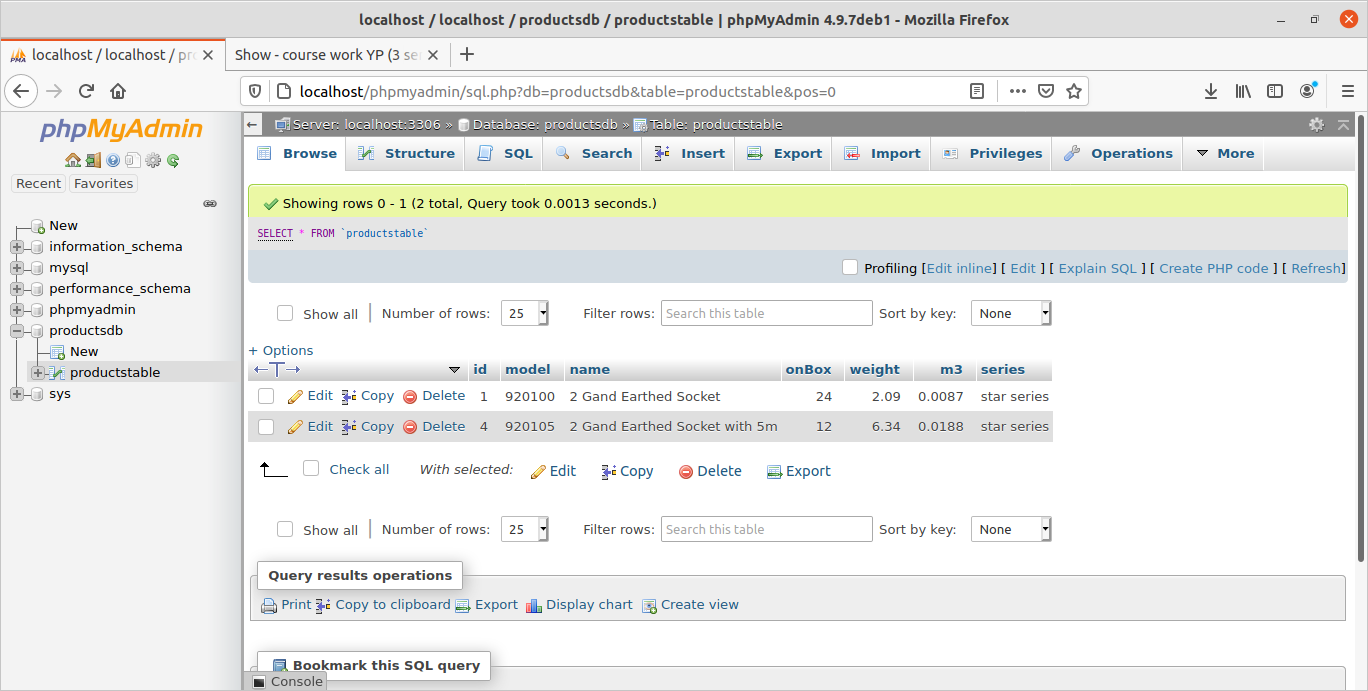
\includegraphics[width=10.5cm]
        {_input/testingTheProgram/checkingTheFunctionsOfTheImplementedSoftware/testDeleteElement/phpmyadmin-after-deleting.png}
    }
    \caption{Таблица phpmyadmin после удаления элемента}
    \label{fig:mysql_table_after_deleting}
\end{figure}

\begin{figure}[p]
    \center{
        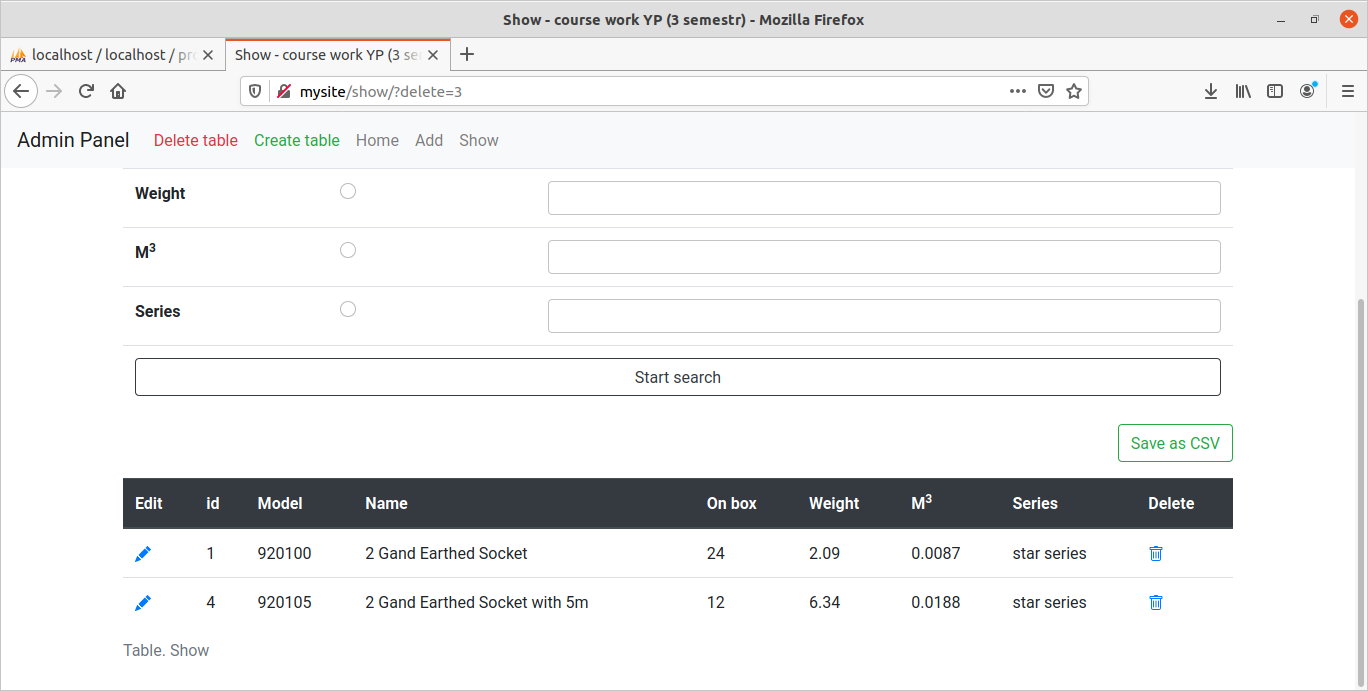
\includegraphics[width=10.5cm]
        {_input/testingTheProgram/checkingTheFunctionsOfTheImplementedSoftware/testDeleteElement/site-after-deleting.png}
    }
    \caption{Вывод таблицы на сайте после удаления элемента}
    \label{fig:site_table_after_deleting}
\end{figure}

\underline{Вывод}:
Удаление элемента из таблицы MySQL через таблицу на сайте по кнопке <<корзина>> работает корректно. Элемент удалился из таблицы под определённым ID. Ожидаемый результат совпал с полученным.

\newpage